%% Diffusion Models in Finance: A Survey — ICAIF submission (ACM sigconf)
%% Full-length (~8pp) version condensed from ../comprehensive-survey.md.
%% Compile: pdflatex main && bibtex main && pdflatex main && pdflatex main
\documentclass[sigconf,nonacm]{acmart}

\usepackage{booktabs}
\usepackage{amsmath}
\usepackage{graphicx}
\usepackage{algorithm}
\usepackage{algpseudocode}
\usepackage{tabularx}
\usepackage{array}
\usepackage{tikz}
\usetikzlibrary{positioning,fit,backgrounds,arrows.meta}

\definecolor{finBlue}{HTML}{2F6F9F}
\definecolor{finTeal}{HTML}{2A9D8F}
\definecolor{finGold}{HTML}{C49A27}
\definecolor{finRed}{HTML}{B55A4A}
\definecolor{finViolet}{HTML}{6D5BA6}
\definecolor{finInk}{HTML}{263238}
\definecolor{finMist}{HTML}{EEF3F6}

\setlength{\textfloatsep}{8pt plus 2pt minus 2pt}
\setlength{\dbltextfloatsep}{8pt plus 2pt minus 2pt}
\setlength{\floatsep}{6pt plus 2pt minus 2pt}
\setlength{\dblfloatsep}{6pt plus 2pt minus 2pt}
\captionsetup{font=small,skip=3pt}
\newcolumntype{Y}{>{\raggedright\arraybackslash}X}

\begin{document}

\title{Diffusion Models in Finance: A Survey}

%% Anonymous review copy. Replace with final author metadata after acceptance.
\author{Anonymous Author(s)}
\affiliation{%
  \institution{Anonymous Institution(s)}
  \country{}}

\renewcommand{\shortauthors}{Anonymous Author(s)}

\begin{abstract}

\end{abstract}

\keywords{diffusion models, score-based generative models, flow matching, finance, survey}

\maketitle

\section{Introduction}

What's the problem? Why people care about this survey? This should be a short background and motivation.

\textbf{Why diffusion, why now.}
Generative modeling is useful in finance because many important regimes are rare,
private, or expensive to observe: market crashes, stressed liquidity, credit
defaults, customer-level fraud, and realistic high-frequency order flow.
Denoising diffusion probabilistic models (DDPMs)~\cite{ho2020ddpm} and
score-based generative models~\cite{song2019ncsn,song2021sde} offer stable
training, strong mode coverage, and flexible conditioning. Those properties make
them attractive for synthetic financial data, scenario generation, forecasting,
and decision support, where GAN-style instability and mode collapse are
especially costly.

\textbf{Contributions.}
We make three contributions. First, we introduce a data-first taxonomy that
organizes diffusion-family finance papers by the object being modeled:
financial time series, limit order books (LOBs), tabular records, and other
structured financial objects. Second, we connect those data domains to common
applications--generation, prediction and inference, trading and portfolio
construction, risk and stress testing, and privacy. Third, we summarize open
problems around benchmarks, tail fidelity, market validity, privacy, and
non-stationarity.

\textbf{Scope and taxonomy of this survey.}
We include learned diffusion, score-based, flow-matching, rectified-flow, and
stochastic-interpolant models when they are applied to financial data or provide
directly relevant backbones. We exclude classical financial ``diffusion''
models in the purely SDE/PDE sense unless they contain a learned generative
sampler. Figure~\ref{fig:taxonomy} shows the organizing principle: the data
object is the primary axis; application and method family are secondary axes.
This differs from generic time-series diffusion surveys~\cite{yang2024tssurvey},
tabular-diffusion surveys~\cite{challagundla2025tabsurvey}, and broad
synthetic-data surveys~\cite{li2025gensynthsurvey}, because finance imposes
domain-specific requirements: no-arbitrage and measure consistency, heavy tails,
stylized facts, microstructure realism, and privacy/governance.

\begin{figure*}[t]
  \centering
  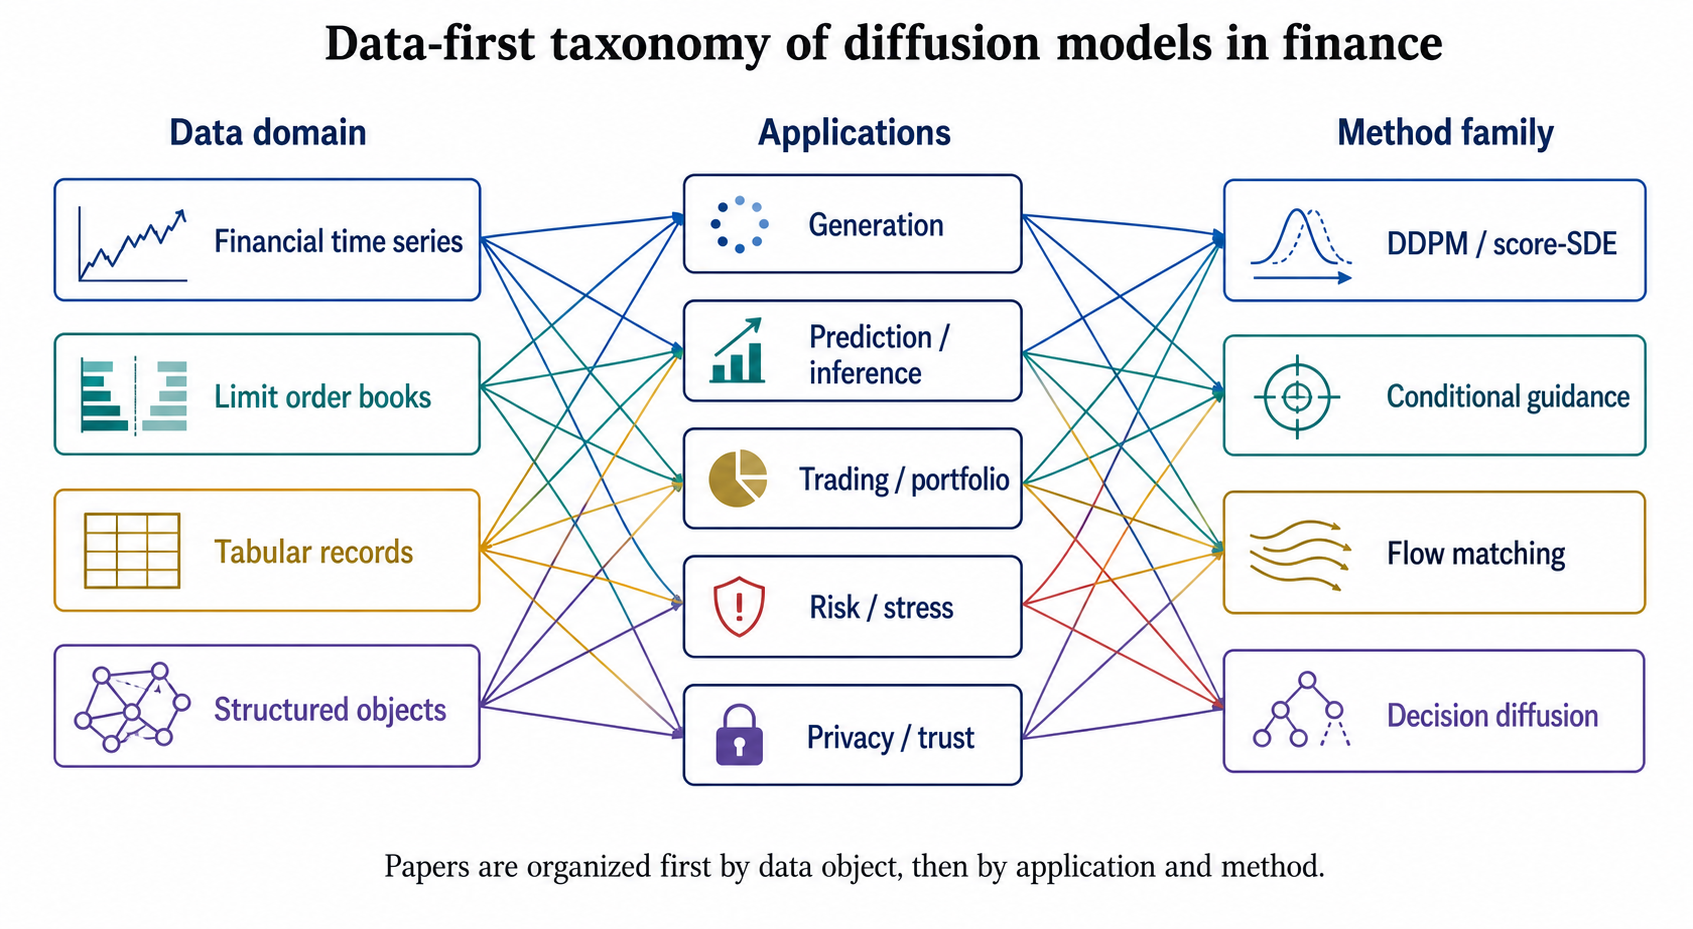
\includegraphics[width=\textwidth]{figures/data_first_taxonomy.png}
  \caption{A data-first taxonomy for diffusion-family models in finance. Papers
  are organized first by the financial data object, then by application and
  method family.}
  \Description{A taxonomy chart linking four financial data domains to major
  applications and diffusion-family method families.}
  \label{fig:taxonomy}
\end{figure*}

The rest of the paper follows the same taxonomy. Section~\ref{sec:bg} gives
background. Sections~\ref{sec:fts}--\ref{sec:structured} review the literature
by data domain. Section~\ref{sec:discussion} discusses cross-cutting trends,
evaluation, open problems, and directions.

\section{Background}\label{sec:bg}
This section fixes the common vocabulary used throughout the survey. We keep the
presentation deliberately compact: the goal is not to re-derive diffusion models,
but to identify the design choices that become consequential once the data are
prices, order books, credit tables, or arbitrage-constrained financial objects.

\textbf{Denoising diffusion and score-based foundations.}
DDPMs define a forward noising process that gradually transforms data
$x_0 \sim p_{\rm data}$ into an approximately Gaussian variable $x_T$,
typically through transitions $q(x_t \mid x_{t-1})$ with a prescribed noise
schedule~\cite{ho2020ddpm}. A neural network is then trained to reverse this
process, often by predicting the injected noise. The practical appeal is that training is stable and uses a
simple denoising objective, while sampling produces diverse draws by running the
learned reverse chain from noise to data. Score-based generative models instead
learn $s_\theta(x,t,c)\approx \nabla_x \log p_t(x\mid c)$ at multiple noise
levels~\cite{song2019ncsn}. The two views meet in the score-SDE formulation~\cite{song2021sde},
where a forward process
\begin{equation}
  d x_t = f_t(x_t)\,dt + g_t\,d w_t
\end{equation}
is sampled in reverse by replacing the unknown score with a neural estimate:
\begin{equation}
  d x_t = \{f_t(x_t)-g_t^2 s_\theta(x_t,t,c)\}\,dt + g_t\,d\bar{w}_t.
\end{equation}
Here $c$ denotes optional conditioning information and $\bar{w}_t$ is the
reverse-time Brownian motion. Training usually samples
$x_0$, a noise level $t$, and a perturbed observation
$x_t=\alpha_t x_0+\sigma_t\epsilon$, then fits either the score or the injected
noise. Algorithm~\ref{alg:sde} gives the resulting template, following standard
score-SDE notation. For finance this connection is
conceptually useful: stochastic processes are already the language of asset
prices, rates, volatility, and risk-neutral valuation. The learned component is
not a classical calibrated diffusion coefficient, but the reverse-time score or
drift that transports a tractable base distribution into an empirical financial
data distribution.

\begin{algorithm}[t]
\caption{Score-SDE diffusion: training and sampling}
\label{alg:sde}
\small
\begin{algorithmic}[1]
\State \textbf{Input:} data $x_0$, optional condition $c$, schedule $(\alpha_t,\sigma_t)$, score/noise network.
\Statex \textit{Training}
\For{each minibatch}
  \State Sample $t\sim U(0,T)$ and $\epsilon\sim\mathcal{N}(0,I)$.
  \State Form $x_t=\alpha_t x_0+\sigma_t\epsilon$.
  \State Minimize $\|s_\theta(x_t,t,c)-\nabla_{x_t}\log p(x_t\mid x_0)\|_2^2$.
  \State Equivalently, under Gaussian paths, minimize $\|\epsilon_\theta(x_t,t,c)-\epsilon\|_2^2$.
\EndFor
\Statex \textit{Sampling}
\State Draw $x_T\sim\mathcal{N}(0,I)$.
\For{$t=T,T-\Delta t,\ldots,\Delta t$}
  \State Draw $z\sim\mathcal{N}(0,I)$.
  \State $x_{t-\Delta t}=x_t-\{f_t(x_t)-g_t^2 s_\theta(x_t,t,c)\}\Delta t+g_t\sqrt{\Delta t}\,z$.
\EndFor
\State \Return synthetic sample $\hat{x}_0$.
\end{algorithmic}
\end{algorithm}


\textbf{Flow matching, rectified flow, and stochastic interpolants.}
Recent work also uses continuous-time transport formulations that learn a vector
field from a base distribution to the data. In its simplest form, flow matching
learns an ODE
\begin{equation}
  \frac{d x_t}{dt}=v_\theta(x_t,t,c), \qquad x_0\sim p_0,
\end{equation}
whose terminal distribution approximates $p_{\rm data}$. With a linear
conditional path $x_t=(1-t)z+t x$ between noise $z\sim p_0$ and data
$x\sim p_{\rm data}$, the target velocity is $u_t=x-z$, giving the objective
\begin{equation}
  \mathcal{L}_{\rm FM}(\theta)=
  \mathbb{E}_{x,z,t}\left[\|v_\theta(x_t,t,c)-(x-z)\|_2^2\right].
\end{equation}
Algorithm~\ref{alg:flow} summarizes the corresponding training and Euler
sampler~\cite{lipman2023flow,holderrieth2026introflowdiffusion}. Rectified flow
straightens the transport path to reduce sampling cost~\cite{liu2023rectifiedflow},
and stochastic interpolants provide a broad framework that contains diffusion and
flow models as special cases~\cite{albergo2023interpolants}.

\begin{algorithm}[t]
\caption{Flow matching: training and sampling}
\label{alg:flow}
\small
\begin{algorithmic}[1]
\State \textbf{Input:} data $x$, base noise $z\sim p_0$, optional condition $c$, vector field $v_\theta$.
\Statex \textit{Training}
\For{each minibatch}
  \State Sample $t\sim U(0,1)$, $z\sim p_0$, and $x\sim p_{\rm data}$.
  \State Set $x_t=(1-t)z+t x$ and target velocity $u_t=x-z$.
  \State Minimize $\|v_\theta(x_t,t,c)-u_t\|_2^2$.
\EndFor
\Statex \textit{Sampling}
\State Draw $x_0\sim p_0$.
\For{$t=0,\Delta t,\ldots,1-\Delta t$}
  \State $x_{t+\Delta t}=x_t+\Delta t\,v_\theta(x_t,t,c)$.
\EndFor
\State \Return synthetic sample $\hat{x}_1$.
\end{algorithmic}
\end{algorithm}

\textbf{Conditioning and guidance.}
Classifier guidance modifies the reverse process using gradients from an auxiliary model,
while classifier-free guidance learns conditional and unconditional scores in a
single model and interpolates them at sampling time~\cite{dhariwal2021beatgan,
ho2022cfg}. Finance papers adapt this idea to regime labels, factor states,
asset identities, missing-value masks, stress intensities, portfolio objectives,
or structural constraints. Conditioning is therefore not a cosmetic add-on: it is
the mechanism that turns a generator into a controllable market simulator,
forecaster, imputer, stress-test engine, or decision module.



\textbf{Sampling accelerators and architectural backbones.}
Sampling speed is a recurring bottleneck. DDIM~\cite{songddim2021}, improved
diffusion objectives~\cite{nichol2021improved}, EDM design choices
~\cite{karras2022edm}, and consistency models~\cite{song2023consistency} seek
better sample quality per function evaluation. In parallel, domain backbones
determine what the model can represent:
TimeGrad handles probabilistic time-series forecasting~\cite{rasul2021timegrad},
CSDI addresses conditional imputation~\cite{tashiro2021csdi}, SSSD combines
diffusion with structured state-space sequence modeling~\cite{alcaraz2022sssd},
TSDiff and Diffusion-TS explore forecasting and interpretable time-series
generation~\cite{kollovieh2023tsdiff,yuan2024diffusionts}, and TabDDPM/TabSyn
adapt diffusion to mixed-type tabular data~\cite{kotelnikov2023tabddpm,
zhang2024tabsyn}. Finance papers typically inherit these ideas, then add
financial structure: asset embeddings, factor conditioning, temporal masks,
privacy mechanisms, no-arbitrage penalties, or microstructure-aware encodings.

\textbf{Decision-making and control.}
Many financial problems are not finished when a realistic sample is generated.
Portfolio construction, hedging, execution, and market making require actions
under uncertainty. Diffusion policies and trajectory generators provide a bridge
from generative modeling to control: Diffuser models behavior trajectories for
planning~\cite{janner2022diffuser}; Decision Diffuser frames conditional
generation as a decision-making primitive~\cite{ajay2022decisiondiffuser}; and
the reinforcement-learning literature surveys diffusion as policy, planner, and
data generator~\cite{zhu2023diff4rl}. In finance, this perspective appears when
synthetic scenarios are used to train robust portfolio policies, when market
generators support trading simulation, or when conditional paths feed pricing and
hedging routines. The modeling question therefore shifts from ``does the sample
look real?'' to ``does the generated distribution support better decisions under
the constraints of the market?''

\begin{table*}[t]
\centering
\caption{Representative diffusion-family finance papers organized by data
domain. The table is illustrative rather than exhaustive; entries are selected
to show the taxonomy used in this survey.}
\label{tab:representative}
\scriptsize
\setlength{\tabcolsep}{2pt}
\begin{tabular}{@{}p{0.22\textwidth}p{0.055\textwidth}p{0.12\textwidth}p{0.17\textwidth}p{0.18\textwidth}p{0.11\textwidth}p{0.045\textwidth}@{}}
\toprule
Paper & Year & Data domain & Region / Asset / Data & Application & Method family & Code \\
\midrule
Beyond Monte Carlo~\cite{lesniewski2024beyondmc} & 2024 & Time series & US / Stock / Return vectors & Market simulation & Diffusion & -- \\
A Financial Time Series Denoiser~\cite{wang2024ftsdenoiser} & 2024 & Time series & US / Stock / Price series & Denoising / trading signal & Conditional diffusion & -- \\
CoFinDiff~\cite{tanaka2025cofindiff} & 2025 & Time series & JP / Stock / Price series & Controllable generation & Conditional diffusion & -- \\
Diffusion Factor Models~\cite{chen2025difffactor} & 2025 & Time series & US / Stock / Return series & Factor-structured returns & Diffusion & Yes \\
TRADES~\cite{berti2025trades} & 2025 & LOB & US / Stock / LOB orderflow & Market simulation & Diffusion & Yes \\
DiffVolume~\cite{wang2025diffvolume} & 2025 & LOB & US / Stock / LOB volume & Volume generation & Diffusion & -- \\
DiffLOB~\cite{wang2026difflob} & 2026 & LOB & US / Stock / LOB snapshots & Counterfactual generation & Diffusion & Yes \\
FinDiff~\cite{sattarov2023findiff} & 2023 & Tabular & Multi / Credit, Payment, Fund / Tabular & Tabular synthesis & Diffusion & Yes \\
Imb-FinDiff~\cite{sattarov2024imbfindiff} & 2024 & Tabular & Multi / Finance / Tabular & Imbalance synthesis & Conditional diffusion & -- \\
DP-FinDiff~\cite{sattarov2025dpfindiff} & 2025 & Tabular & Multi / Finance / Tabular & Private synthesis & DP diffusion & Yes \\
IV-surface diffusion~\cite{jin2025ivsurface} & 2025 & Structured & US / Option / IV surface & Surface forecasting & Diffusion & Yes \\
Risk-neutral derivative pricing~\cite{tiwari2026riskneutral} & 2026 & Structured & Global / Stock / Return series & Derivative pricing & Diffusion & -- \\
\bottomrule
\end{tabular}
\end{table*}

Figure~\ref{fig:coverage} summarizes the same corpus at a coarser level,
showing where diffusion-family finance papers cluster and where coverage remains
thin.

\begin{figure*}[t]
  \centering
  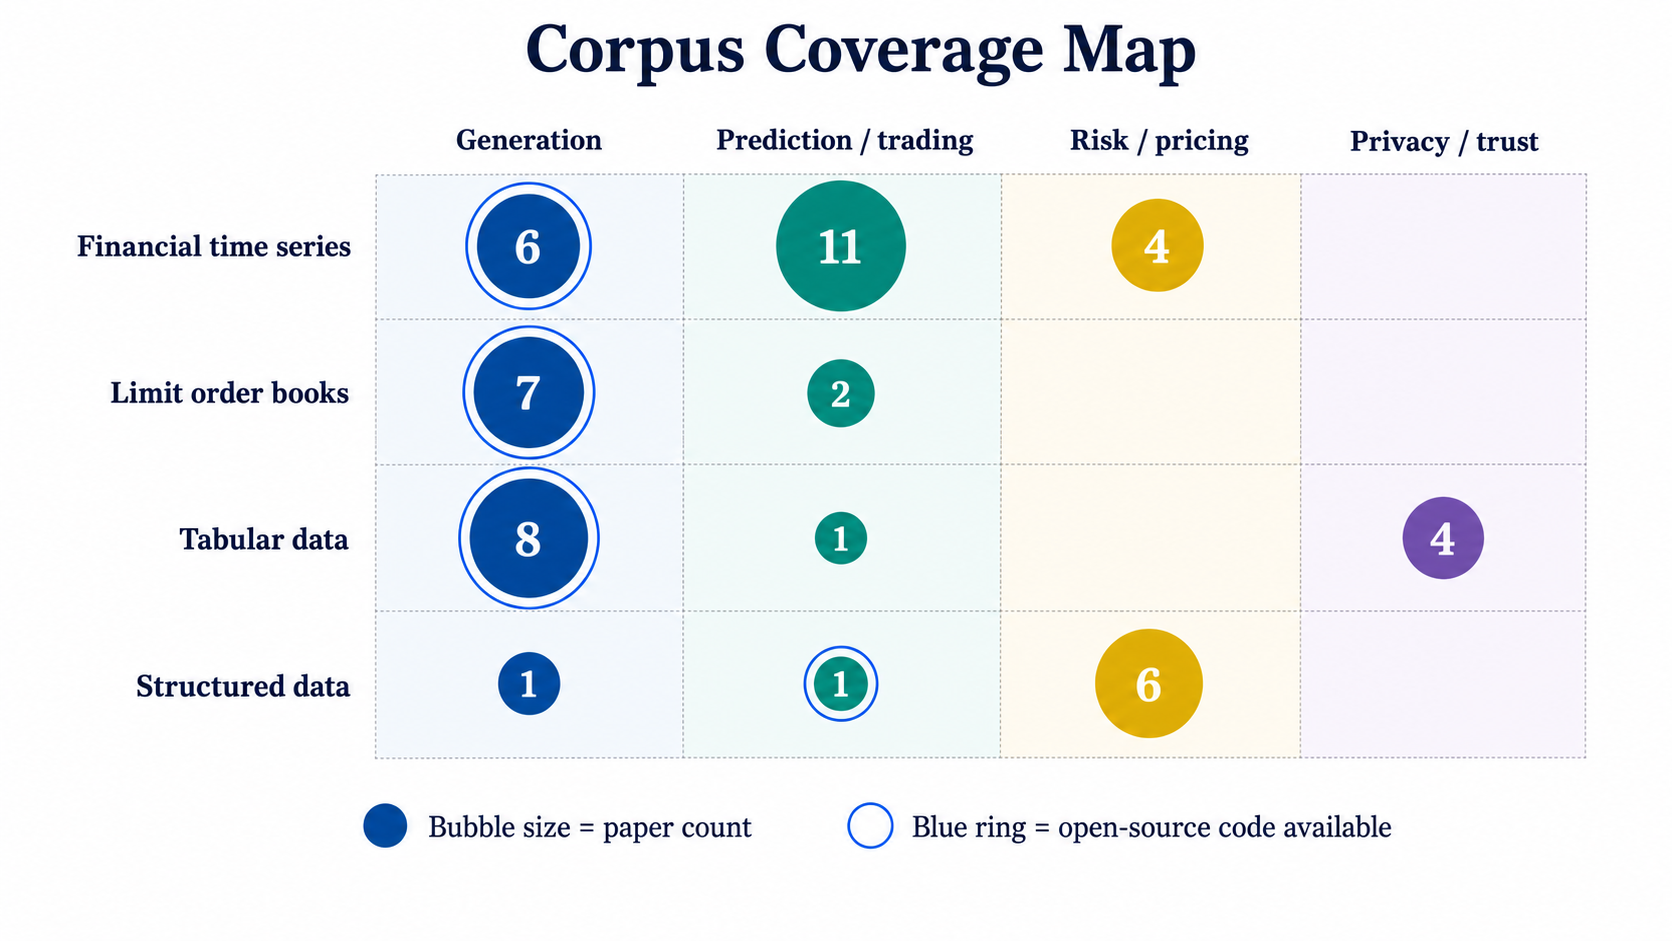
\includegraphics[width=0.92\textwidth]{figures/corpus_coverage_map.png}
  \caption{Corpus coverage map by financial data object and application. Cell
  numbers count finance-facing corpus entries; bubble size encodes paper count,
  and blue rings indicate cells with public implementations. Cross-listed papers
  may appear in multiple cells.}
  \Description{A heatmap with rows for time series, limit order books, tabular
  data, and structured financial data, and columns for generation, prediction and
  trading, risk and pricing, and privacy and trust.}
  \label{fig:coverage}
\end{figure*}

\section{Financial Time Series Data}\label{sec:fts}

% Give a general overview of this section. 
Financial time series form the largest cluster in the current literature. In
this section, we use the term narrowly: the modeled object is an ordered sequence
such as prices, returns, macroeconomic variables, etc. We therefore separate this section from
LOBs in next section, where the sequence is constrained by order-book mechanics, and from
structured objects such as implied-volatility surfaces or yield curves. The
dominant assets are equities and ETFs, with smaller coverage of futures, energy
prices, and macro-conditioned paths. Across these settings, the generator must
preserve stylized facts that ordinary time-series metrics often miss, such as heavy
tails, volatility clustering, leverage effects, serial dependence and cross-sectional covariance.

Two modeling choices recur. First, papers decide whether to model prices or
returns. Price paths are visually and economically intuitive, but they are
non-stationary and scale-sensitive; return series are closer to stationary and
portfolio-ready, but harder to evaluate visually and easier to over-smooth.
Second, papers decide whether the diffusion model is the final product or an
intermediate object. Some works output synthetic paths for simulation or data
sharing. Others use diffusion as a probabilistic forecaster, scenario
tree generator, denoiser, or policy-training environment.

\subsection{Unconditional Generation}\label{sec:fts-uncond}

Unconditional generation asks whether a model can synthesize financial time
series without specifying a future condition, regime, or control signal. We read
these papers along two axes: the financial variable being generated and the
dimensionality of the generated object. The variable axis separates price or
price-like paths from returns, return vectors, spreads, volumes, and transformed
market features. The dimensionality axis separates single-instrument generation
from multivariate panels that must preserve cross-asset dependence. 

Most unconditional finance papers in the current corpus are stock-market papers.
Takahashi and Mizuno use US intraday stock data and generate a single-stock,
multivariate-feature time series: price log returns, spreads, and trading volumes
are converted to wavelet images and reconstructed as synthetic market series
~\cite{takahashi2024synthfts}. Lesniewski and Trigila use US equity data, but
the generated object is not a price path; it is a multivariate stock-return
scenario used for covariance regularization and portfolio-level simulation
~\cite{lesniewski2024beyondmc}. Diffusion Factor Models move to high-dimensional
stock-return panels, generating multivariate asset returns under a latent factor
structure rather than independent univariate series~\cite{chen2025difffactor}.
Kim et al. use historical stock data and generate price-path-oriented series with
a GBM-informed noising process, making the model closer to price dynamics than
return-only scenario generation~\cite{kim2025gbmdiff}. Fiaingen is useful as a
stock-data-quality reference point: it works with daily stock closing-price
windows and evaluates whether generated stock time series support downstream
learning, although it is better treated as a synthetic-data comparator than as a
core diffusion architecture~\cite{rozanec2025fiaingen}.

\subsection{Conditional Generation}\label{sec:fts-cond}
Conditional generation asks whether a model can synthesize financial time series
under an observed or user-specified condition. Compared with unconditional
generation, the key question is not only what variable is generated, but also
what information controls the generation. We read this literature along two
axes: the generated data object, such as prices, returns, charts, or scenario
paths, and the conditioning signal, such as trend, volatility, partial
observations, stress regimes, or optimization states. This distinction is
important because conditional generators are usually evaluated by whether they
respond correctly to the condition, not only by whether their samples look
realistic on average.

For stock data, conditional generation mainly appears as controllable stock
time-series synthesis and stress-scenario construction. CoFinDiff uses Japanese
stock price series and generates multivariate stock time series conditioned on
user-specified trend and volatility controls, so the generated object is
price-like stock series rather than return-only scenarios~\cite{tanaka2025cofindiff}.
Diffusion-Augmented Reinforcement Learning uses stock-market return scenarios
conditioned toward crash or stress regimes; the generated data are multivariate
stock-return paths used to train robust portfolio policies rather than generic
synthetic prices~\cite{choudhary2025diffaugrl}. ~\citet{guo2025compressedsensing} uses financial time-series observations under partial or
compressed measurements and reconstructs plausible stock and macro time-series
signals, making the generated object a conditionally completed financial series
rather than an unconditional market sample.

Outside stocks, conditional generation becomes more heterogeneous. Chart-based
diffusion forecasting represents financial time series as visual chart objects
and generates future chart continuations, with the experiments centered on
Bitcoin futures price charts rather than equity panels~\cite{lee2025charts}.
Scenario-tree generation uses multivariate energy price time series and generates
conditional scenario paths for multistage stochastic optimization, so the data
object is an optimization-ready scenario tree rather than a simple price
sequence~\cite{zarifis2025scenariotree}. These papers show why conditional
generation should be separated from unconditional synthesis: the generated data
must be realistic, but it must also be coherent with the conditioning signal and
useful for the downstream decision problem.

\subsection{Prediction and Trading}\label{sec:fts-decision}

Prediction-oriented papers use diffusion models to forecast future financial
states or to construct signals that feed trading and allocation decisions. In
this subsection, prediction includes point or distributional forecasts of prices,
returns, chart movements, denoised signals, portfolio weights, and trading
actions. This boundary is useful because finance rarely evaluates prediction in
isolation: a forecast is valuable only if it improves trading accuracy,
risk-adjusted return, drawdown control, or portfolio robustness. Thus the central
question is not only whether the generated distribution is realistic, but whether
it is decision-useful under chronological splits, transaction costs, and changing
market regimes.

Stock-level prediction papers mostly use diffusion as a way to denoise, augment,
or represent financial time-series signals. \citet{wang2024ftsdenoiser} use US
stock price series and apply a diffusion denoiser to financial time-series
signals before downstream prediction and trading evaluation. \citet{daiya2024diffstock}
use US stock relational time-series data and generate probabilistic stock-market
predictions, making the modeled object a cross-sectional prediction distribution
rather than a standalone synthetic series. \citet{gao2024diffsformer} use Chinese
stock factor and price-related data, with diffusion-based factor augmentation
serving the prediction model rather than general market simulation.
\citet{lee2025charts} recast financial forecasting as conditional image
generation: historical price charts are treated as visual inputs, and a
text-to-image diffusion model generates the next chart image to predict future
price trends. These papers differ in representation, but they share the same
evaluation burden: the diffusion component must improve prediction or trading
signals beyond a strong chronological baseline.

Portfolio and trading papers move from forecasting signals to decision variables.
\citet{cho2025diffolio} model multivariate financial time series and generate
predictive return distributions for portfolio construction, so the relevant data
object is a multivariate return distribution rather than a single price path.
\citet{gao2025factorcond} condition stock-return generation on asset-specific
factors and use the resulting samples for constrained mean-variance and
mean-CVaR portfolio optimization. \citet{alzahrani2025marcd} focus on
regime-aware and tail-risk-sensitive return scenarios for CVaR-constrained
portfolio decisions, making the generated distribution explicitly risk-driven.
\citet{choudhary2025diffaugrl} generate stress-oriented stock-return scenarios to
train robust portfolio reinforcement-learning policies. \citet{li2025flowhft}
shift the prediction-decision link to high-frequency trading, where flow matching
is used inside an imitation-learning policy under diverse market states. Across
these works, the strongest evidence is not sample realism alone, but whether the
diffusion-generated forecast, scenario, or policy improves realized financial
decisions after costs, constraints, and regime changes are considered.

\section{Limit Order Book Data}\label{sec:lob}

Limit order book (LOB) data describe the visible supply and demand around the
best bid and ask through price levels, queue sizes, order arrivals, cancellations,
and trades. Unlike daily financial time series, LOB data are event-driven,
high-dimensional, and constrained by market mechanics: prices must respect tick
sizes, bid prices must remain below ask prices, queue sizes are nonnegative, and
order flow must evolve in a temporally coherent way. These constraints make LOB
generation more difficult than generic multivariate time-series synthesis. A
useful split is therefore between papers that build generative market simulators
and papers that use diffusion models for LOB prediction or forecasting.

\subsection{Generative Market Simulation}\label{sec:lob-sim}

Generative LOB papers aim to synthesize realistic order-book states, event
streams, or market responses. \citet{berti2025trades} use US stock LOB order-flow
data and generate realistic event-level market simulations with a diffusion
model, making the data object an order-flow trajectory rather than a daily price
series. \citet{wang2025diffvolume} focus on US stock LOB volume and generate
conditional volume profiles inside the order book, so the modeled variable is
queue volume rather than the full event stream. \citet{backhouse2025painting}
represent US stock LOB snapshots as image-like structures and use diffusion for
market simulation, with the generated object being book states over time.
ByteGen works at the orderbook-event level but uses a tokenizer-free byte-space
generator, making it useful context for event-stream generation even though its
architecture is not a standard diffusion model~\cite{li2025bytegen}.
\citet{huang2024digma} generate controllable Chinese stock-market order flow with
a diffusion-guided meta-agent, placing the emphasis on market-state control and
agent-based simulation. \citet{wang2026difflob} use US stock LOB snapshots and
generate counterfactual order-book trajectories under regime controls, so the
central object is a controllable LOB state path rather than a point forecast.

\subsection{Prediction}\label{sec:lob-pred}

LOB prediction papers use diffusion models to infer future event streams or book
states from recent market history. \citet{zheng2024lobdif} provide the clearest
prediction-focused example: they use US and Chinese stock LOB order-flow data and
model the joint distribution of future event types and event times, making the
generated object a future LOB event stream. The prediction target is therefore
not a synthetic market for offline simulation, but the next sequence of
high-frequency order-book events. \citet{backhouse2025painting} also connect LOB
generation to forecasting by treating order-book states as structured
image-like data and evaluating future book reconstruction. These papers suggest
that diffusion-based LOB prediction should be evaluated differently from daily
return forecasting: beyond directional accuracy, it must preserve event timing,
queue dynamics, price-level constraints, and the short-horizon structure that
trading systems actually consume.

\section{Tabular Data}\label{sec:tabular}

Financial tabular data consist of row-wise records such as credit applications,
payment transactions, customer attributes, fund characteristics, fraud labels,
and account-level features. Unlike financial time series or LOBs, these data are
usually mixed-type: continuous fields, categorical variables, binary indicators,
timestamps, labels, and entity identifiers may appear in the same table. The
main modeling challenge is therefore not temporal coherence, but preserving
feature-label relationships, categorical distributions, business constraints,
rare classes, and privacy. We organize this section by the motivation for
generation: synthesis and augmentation for utility, and privacy and
trustworthiness for safe deployment.

\subsection{Synthesis and Augmentation}\label{sec:tabular-synthesis}

The first group of tabular papers uses diffusion or flow models to generate
synthetic financial records that can replace, supplement, or rebalance real
training data. \citet{sattarov2023findiff} propose FinDiff for financial tabular
data generation, targeting mixed financial records such as credit, payment, and
fund-like tables. The generated object is a synthetic row with heterogeneous
features, so evaluation must check both marginal feature realism and joint
feature-label consistency. Entity-based financial tabular synthesis extends this
idea to entity-structured records, where generated rows must remain plausible
within the attributes and relationships of financial entities
~\cite{liu2024enttabdiff}. \citet{sattarov2024imbfindiff} focus on class imbalance:
their conditional diffusion model generates minority-class financial records so
that downstream classifiers can learn rare but important events. Flow-based
latent-space augmentation work follows the same utility-driven logic, using
latent diffusion/flow samples to improve prediction on credit and customer
tabular tasks~\cite{ihsan2025latentflow}. \citet{kuo2026emdt} apply a diffusion
transformer to fraud-detection tables, where the generated records are useful
only if they improve rare-event detection without distorting the fraud/non-fraud
boundary.

\subsection{Privacy and Trustworthiness}\label{sec:tabular-privacy}

The second group treats synthetic tabular data as a privacy- and
trust-constrained object. Financial institutions often cannot share raw customer,
transaction, or credit records, so synthetic data are valuable only if they
retain utility while reducing memorization and disclosure risk. Federated
diffusion with differential privacy addresses this setting by learning tabular
generators across decentralized financial datasets while limiting information
leakage from any participant~\cite{sattarov2024dpfedtabdiff}. Privacy-preserving
mixed-type diffusion models make the same concern explicit for heterogeneous
financial tables, where leakage may occur through rare categorical combinations
as well as continuous outliers~\cite{sattarov2025dpfindiff}. Measuring privacy
risks and tradeoffs in financial synthetic data generation shifts the emphasis
from model design to evaluation: utility, fidelity, and disclosure risk must be
reported together rather than optimized separately~\cite{zuo2026privacyrisks}.
Across these papers, the core benchmark is a privacy-utility-trust triangle:
generated tables should help downstream models, avoid leaking sensitive records,
and satisfy the structural rules that make financial records credible.

\section{Other Structured Financial Data}\label{sec:structured}

Not all financial objects are ordinary time series, LOB states, or tabular rows.
Some data objects carry mathematical structure that must be preserved by the
generator. Examples include correlation matrices, implied-volatility surfaces,
yield curves, derivative paths, and risk-neutral pricing objects. These objects
are structured because validity is partly defined by financial constraints:
correlation matrices should be symmetric and positive semidefinite, volatility
surfaces should respect no-arbitrage and cross-maturity consistency, yield curves
should remain smooth and economically plausible, and derivative paths may need to
respect payoff or risk-neutral dynamics. For this reason, evaluation in this
section is less about generic sample realism and more about whether generated
objects remain financially admissible.

Matrix, surface, and curve papers make this constraint issue explicit.
\citet{kubiak2024corrddpm} generate realistic financial correlation matrices
with a DDPM, so the modeled object is not a price or return sequence but a
structured dependence matrix used in portfolio and risk applications.
\citet{jin2025ivsurface} forecast implied-volatility surfaces with generative
diffusion models, where the generated object is a surface over strike and
maturity rather than a one-dimensional volatility series. Term-structure work
uses diffusion models to generate yield curves across maturities, making the data
object a cross-maturity curve whose quality depends on smoothness, level-slope-
curvature structure, and economic plausibility~\cite{fukunishi2025termstructure}.
Across these papers, the challenge is that a generated object can look plausible
under distributional metrics while still violating the financial structure that
makes it useful.

Derivative-path and pricing papers use diffusion models for valuation-oriented
structured data. \citet{zhao2025exotic} apply conditional diffusion to exotic
option valuation and counterparty games, where generated paths must remain
consistent with payoff conditions and valuation objectives. \citet{gao2025sdepaths}
generate solution paths of Markovian stochastic differential equations using
diffusion models, placing the emphasis on path generation under specified
stochastic dynamics rather than empirical market-data synthesis. Risk-neutral
derivative-pricing work uses generative diffusion to approximate pricing
distributions under risk-neutral measures, so the generated object is tied to
valuation rather than ordinary historical forecasting~\cite{tiwari2026riskneutral}.
These papers are best separated from generic financial time-series generation
because their success depends on pricing consistency, path constraints, and
financial admissibility, not only on temporal realism.

\section{Discussion and Conclusion}\label{sec:discussion}

Across the reviewed literature, the central pattern is not simply that diffusion
models can be applied to finance, but that financial generation is becoming
data-object specific. A return panel, a limit order book, a credit table, an
implied-volatility surface, and a risk-neutral path are not interchangeable
arrays. Each carries its own notion of validity: time-series generators must
preserve tails, volatility clustering, co-movement, and regime shifts; LOB
generators must respect event timing, queue dynamics, tick-size rules, and market
response; tabular generators must preserve feature-label relationships while
controlling privacy and rare-class behavior; structured-data generators must
respect positive semidefiniteness, no-arbitrage restrictions, curve smoothness,
or valuation consistency. This data-first view explains why model families alone
are an insufficient taxonomy. The same denoising or flow-matching backbone can be
credible in one domain and unusable in another if it violates the financial
structure of the object being generated.

The most urgent open problem is benchmark and evaluation discipline. Diffusion
models in image, video, and language generation became cumulative partly because
the community built shared datasets, standard protocols, visible leaderboards,
and increasingly demanding evaluation suites. Finance does not yet have an
equivalent. Many papers use proprietary data, incompatible horizons, different
preprocessing choices, weak or non-overlapping baselines, and downstream tasks
that are difficult to compare. As a result, the field risks producing many
plausible demonstrations but little cumulative evidence. A useful research agenda
is to build benchmarks by financial data object: time-series benchmarks should
test tails, volatility clustering, cross-asset dependence, regime robustness, and
portfolio utility; LOB benchmarks should test event timing, queue consistency,
price-level validity, and response to market actions; tabular benchmarks should
jointly report fidelity, privacy leakage, constraint satisfaction, and
minority-class utility; structured-data benchmarks should test positive
semidefiniteness, no-arbitrage, term-structure coherence, and pricing
consistency. Such benchmarks should also include chronological splits,
transaction costs, stress periods, and ablations against strong non-diffusion
models, so that improvement means financial usefulness rather than only sample
realism.

A second open direction is scaling. In images, video, and language, diffusion
models improved through larger corpora, stronger backbones, conditioning,
guidance, representation learning, distillation, and faster samplers. Finance has
not yet had an analogous scaling moment. The obstacles are real: high-quality
financial data are proprietary, fragmented across venues and institutions,
non-stationary across regimes, constrained by regulation, and expensive to label
or release. Yet the opportunity is equally large. Scaled financial generators
could simulate rare regimes, stress portfolios, augment scarce credit and fraud
events, generate coherent order-book worlds, price structured products, and serve
as environment models for trading and risk agents. The next phase of diffusion
models in finance should therefore move beyond asking whether diffusion can
generate financial data, and instead ask whether benchmarked, scaled, and
constraint-aware generators can become trustworthy financial simulators and
decision engines.

This survey argues for a data-first view of diffusion models in finance.
Progress will not come from treating finance as another generic data modality or
from comparing model families in isolation. It will come from building
benchmarked, scaled, and constraint-aware generators whose validity is defined by
the financial object they model. The next phase of diffusion models in finance
should therefore move beyond asking whether diffusion can generate financial
data, and instead ask whether such models can become trustworthy financial
simulators and decision engines.

\bibliographystyle{ACM-Reference-Format}
\bibliography{references}

\end{document}
